% Speech that Protects a Model -- IWAI 2026 camera-ready (LNCS, 12 pages main text + appendix)
\documentclass[runningheads]{llncs}
\usepackage[T1]{fontenc}
\usepackage[utf8]{inputenc}
\usepackage{graphicx}
\usepackage{amsmath,amssymb}
\usepackage{booktabs}
\usepackage{array}
\usepackage{url}
\usepackage[hidelinks]{hyperref}
\usepackage{microtype}
\usepackage{xcolor}
\renewcommand\UrlFont{\color{blue}\rmfamily\small}
\newcommand{\Iw}{I_{\omega}}
\newcommand{\Etrue}{p_{\mathrm{true}}}
\setlength{\tabcolsep}{4pt}

\begin{document}

\title{Speech that Protects a Model: Typed Speech Evidence and Belief-Protecting Mechanisms in a Dialogue Dyad}
\titlerunning{Speech that Protects a Model}
\author{Maria Svet\inst{1}}
\authorrunning{M. Svet}
\institute{Mindloom Cognitive Lab, \href{https://orcid.org/0009-0007-5934-6531}{ORCID 0009-0007-5934-6531}\\ \email{info@mindloom.ch}\\
\url{https://github.com/muqali2816/mindloom_IWAI_2026_speech_protects_model}}

\maketitle

\begin{abstract}
Active-inference accounts of communication explain how dialogue aligns generative models. We ask the converse: how can an exchange continue for many turns and leave a significant expectation unrevised, and what would speech have to make observable for that protection to be attributed rather than presumed? The paper has three parts. (i)~A typed annotation scheme (Mindloom) specifies evidence requirements for ten labels; re-scoring 169 archived cases gives macro-F1 0.757 for the typed engine, 0.837 for a direct language-model prompt and 0.195 for keyword rules tuned on the same cases, which supports an inspectable annotation proposal, not superior classification. (ii)~A single-agent active-inference model shows that weak evidence sensitivity ($\omega$) and a cost of public concession ($c$) produce the same late non-concession (0.989 vs 0.990) with different final belief in the truth (0.538 vs 0.809). (iii)~A new dyadic model connects the parts: a partner's act is evidence, and the \emph{form} of a move---inviting or restricting joint verification---gates whether shared evidence arrives. A third mechanism, aversion to public contradiction ($\gamma$), leaves belief updating intact but reduces what is checked (2.09 vs 2.64 shared signals per dialogue). Each mechanism has one cheap measurement (12--17 simulated dialogues per group) while non-concession alone needs 200. Fed through the archived confusion rows of the typed engine as a noisy channel, invite/restrict labels raise mechanism recovery by 6--8 points over acts alone, whereas labels that only re-encode the act add exactly zero. All bridge results are simulations of stipulated mechanisms; we state which measurements in real dyads would test them.
\keywords{protective speech \and dialogue annotation \and active inference \and belief updating \and mechanism recovery \and dyadic models}
\end{abstract}

\section{Introduction}
Friston and Frith model reciprocal signalling under a shared generative model~\cite{friston2015duet} and extend the account to learning: interaction changes the models through which agents predict each other~\cite{friston2015hermeneutics}. Friston, Parr and colleagues model questions and answers through which one agent's responses become evidence for another~\cite{friston2020linguistic}; Tison and Poirier treat communication as socially extended inference~\cite{tison2021communication}; Medrano and Sajid show multistable dyadic dynamics~\cite{medrano2024broken}. These are accounts of how dialogue supports coordinated inference. We ask a complementary question: what happens when interaction continues but the relevant experience does not lead a participant to revise a significant expectation? A speaker may change the subject, discredit the source, demand reassurance or close the exchange. Our hypothesis is that such moves can \emph{protect} an internal model---reorganise the dialogue so that an expectation that could be reconsidered is not---and that sustained protection may require \emph{compensatory} regulation with a cost~\cite{svet2026paperI,svet2026paperII}. This is a proposed pathway to test, not a result established here.

\paragraph{One situation, two trajectories.} The following constructed exchanges (not benchmark cases) begin identically. Alex: ``I sent the revised budget with the latest prices.'' Sam: ``The attachment is version~3, with the April prices; version~4 has the May prices.'' In trajectory~A Alex replies ``Can we compare the files? I thought I had attached version~4,'' Sam shows the attachment, Alex concedes and proposes a check next time. In trajectory~B Alex replies ``You always look for mistakes in my work,'' then ``I know what I sent. If you trusted me, you would stop questioning this,'' and Sam gives up: ``There is no point showing you the file.'' The two trajectories differ in two things at once. First, in what is \emph{said} (a concession is or is not made). Second, in the \emph{form} of the moves: A \emph{invites} joint verification---the attachment becomes a shared object of inspection---while B \emph{restricts} it: further questioning is made incompatible with trust, and the check is abandoned. Crucially, B does not reveal whether Alex privately changed their mind. The same public stance can accompany weak belief updating, a changed belief that is costly to acknowledge, or an intact updater who arranges for nothing to be checked.

\paragraph{Contributions and what is not claimed.} Part~I (Sect.~\ref{sec:part1}) specifies what speech makes observable and how reliably archived systems recover it, now with a keyword baseline and a benchmark-construction table. Part~II (Sect.~\ref{sec:part2}) shows in a single-agent active-inference model that public non-concession cannot separate weak updating from costly concession, and which observations can. Section~\ref{sec:bridge} is new: a hybrid dyadic model in which speech is evidence for the partner \emph{and} controls access to joint verification, with the Part~I labels entering as a noisy measurement channel. The model formalises the invite/restrict distinction of the example above and yields a third mechanism---access protection---that is publicly indistinguishable from honesty on non-concession. Everything in Sections~\ref{sec:part2}--\ref{sec:bridge} is simulation of stipulated mechanisms; no human data enter, no psychological regime is validated and no physiological cost is measured. The labels are \emph{descriptive targets}; whether any has the hypothesised protective function is what the dyadic model says one would have to measure.

\section{Part I: Describing speech with explicit evidence}
\label{sec:part1}
\subsection{Annotation objects}
Mindloom annotates a speaker's contribution in its supplied context. The engine passes through five layers: L1 records surface evidence atoms (a named feeling, a question form, an absolute expression), L2 aggregates them into evidence features, L3 checks evidence requirements (``bridges'') that each label must satisfy, L4 assigns at most one configuration and L5 emits the typed output with the evidence trail or abstains with \emph{insufficient context}. Table~\ref{tab:labels} lists the ten labels. Eight are \emph{configurations} of a single contribution; SEAL is a \emph{function} (closure) that can co-occur with a configuration; SHIFT is an \emph{event} requiring before-and-after configuration evidence. The two labels that carry the invite/restrict contrast used later are SEEK (inquiry that makes an answer relevant) and LOCK (language constraining the addressee's acceptable replies). SEAL differs from LOCK in scope: SEAL closes a topic or channel (``we're done''); LOCK keeps the channel open but constrains what may be said in it. Labels were historically called regimes; temporal-regime status is not established, and definitions concern \emph{what is said}, not motive.

\begin{table}[t]
\centering\caption{Annotation targets. The wording states the descriptive target only; no label presumes an intent.}
\label{tab:labels}
\footnotesize
\begin{tabular}{@{}llp{7.6cm}@{}}
\toprule
type & label & descriptive target\\
\midrule
configuration & BUILD & joint elaboration or repair with a response still available\\
configuration & SEEK & inquiry that makes an answer relevant\\
configuration & UNSEAL & first-person disclosure without requiring the other to regulate it\\
configuration & LOCK & language constraining the addressee's acceptable replies\\
configuration & DRAIN & the other positioned as a required source of support or regulation\\
configuration & FLOOD & intensification or repetition dominating the exchange\\
configuration & EDGE & alternation between approach and withdrawal\\
configuration & VOID & withdrawal from an offered opportunity to respond\\
function & SEAL & closure of a topic or channel\\
event & SHIFT & change supported by before-and-after configuration evidence\\
\bottomrule
\end{tabular}
\end{table}

\subsection{Benchmark construction}
Reviewers asked how the benchmark was built. Table~\ref{tab:bench} gives the construction facts recomputable from the case files. All 589 cases are English monologue fragments generated for the ontology and coordinator-locked before any run; there are no observed conversations and no full dialogues. Tier~A (169 cases, 35--71 words) contains the ten primary-output labels; Tier~B (420 cases, 1--47 words) tests defence recall only. Tier~A has no exact or near-duplicate texts; Tier~B contains 15 near-duplicate pairs (word 5-gram Jaccard $\ge 0.3$, 3.6\,\% of cases), which we report rather than remove. Case provenance, independent adjudication and separation from ontology development are incompletely documented; the benchmark is an internal curated evaluation whose independence from design choices has not been established. A six-rater pilot on evidence features (not on labels) gave Fleiss' $\kappa$ of 1.00 for lexically direct features (named feeling, explicit return time) and 0.23, 0.13 and $-0.11$ for minimal response, absolute expressions and required response respectively; raw rater matrices are unavailable, so these are transcribed values~\cite{krippendorff2004reliability,passonneau2006masi}.

\begin{table}[t]
\centering\caption{Benchmark construction, recomputed from the case files. Sources: Tier A \texttt{ood\_regime\_200}; Tier B \texttt{defense\_4mon}, \texttt{ood\_defense\_200}. Near-duplicates: word 5-gram Jaccard $\ge0.3$.}
\label{tab:bench}
\footnotesize
\begin{tabular}{@{}lrlrrr@{}}
\toprule
tier & cases & document type & words min/med/max & exact dup. & near-dup. pairs\\
\midrule
A & 169 & monologue fragment & 35 / 50 / 71 & 0 & 0\\
B & 420 & monologue fragment & 1 / 15 / 47 & 0 & 15\\
\bottomrule
\end{tabular}
\end{table}

\subsection{Re-scoring archived classification and baselines}
We re-score the 169 Tier~A cases from three stored predictions per case for the typed engine and a direct-prompt baseline (same model family; the baseline JSON identifies Claude Haiku~4.5, the engine archive carries no provider field); label majority decides, run~0 breaks three-way ties; no new model calls were made. To answer whether the labels are recoverable from surface lexis, we add a rule-based keyword classifier whose patterns were written from the Table~\ref{tab:labels} definitions and then revised three times after inspecting their output on the same 169 cases (no held-out set exists); its score is therefore tuned on the test cases and is an \emph{upper bound} for such a system, not an independent baseline. Majority-class and uniform-random baselines complete Table~\ref{tab:scores}.

\begin{table}[t]
\centering\caption{Strict classification on the July 2026 archive, 169 Tier~A cases. Macro-F1 averages the ten gold categories; non-SHIFT excludes the 20 transition cases.}
\label{tab:scores}
\footnotesize
\begin{tabular}{@{}lrrrr@{}}
\toprule
system & all & non-SHIFT & macro-F1 & SHIFT\\
\midrule
direct prompt (majority of 3) & 145/169 & 127/149 & 0.837 & 18/20\\
typed engine (majority of 3) & 129/169 & 127/149 & 0.757 & 2/20\\
keyword rules (revised on test cases) & 43/169 & 43/149 & 0.195 & 0/20\\
majority class (BUILD) & 20/169 & 20/149 & 0.021 & 0/20\\
uniform random (seed 0) & 17/169 & 14/149 & 0.099 & 3/20\\
\bottomrule
\end{tabular}
\end{table}

The direct prompt is better overall and the two systems tie without SHIFT: the engine has no demonstrated accuracy advantage; its proposed value is the inspectable relation between evidence and output. The keyword rules sit far below both (0.25 accuracy even after tuning on the scored cases), so the labels are not recoverable from simple surface lexis in these 35--71-word fragments, but this is not evidence that the engine's evidence gates are what produces its accuracy: an ablation of gates at a fixed model and prompt was not run. SHIFT is fragile: majority voting returns SEEK for 17 of 20 transition cases; run~0 abstains on 15 of them while runs~1--2 never abstain. The archived gates-off capture shows 17 of 65 manipulation-label emissions citing a bridge whose required evidence was absent from the segment's L1 record; the claim that the gated run removed all 17 is author-reported and not recomputable from the released package. The engine's confusion rows for gold LOCK (10 LOCK, 3 SEAL, 2 BUILD) and gold SEEK (20 SEEK) are reused in Sect.~\ref{sec:bridge} as the noise model of the invite/restrict channel.

\section{Part II: A single-agent test of competing mechanisms}
\label{sec:part2}
Even a perfectly observed refusal to concede leaves its cause open. We compare two mechanisms that preserve public non-concession: \emph{attenuation} of evidence and a \emph{cost of public concession}.

\subsection{Generative model}
The hidden state $x\in\{0,1\}$ says whether the speaker's original position is true. Worlds draw $x$ with probability $0.5$; the speaker starts at $q_0=Q(x{=}1)=0.75$. Each round an observation $e\in\{0,1,\varnothing\}$ opposes the position, supports it, or is absent. The objective likelihood is
\begin{equation}
A_\lambda(e\mid x)=\begin{cases}\lambda\rho & e \text{ matches } x\\ \lambda(1-\rho) & e \text{ opposes } x\\ 1-\lambda & e=\varnothing,\end{cases}\qquad \rho=0.75,
\label{eq:A}
\end{equation}
with arrival rate $\lambda_0=0.35$, or $\lambda_1=0.90$ in the round after an ASK. The speaker's subjective likelihood tempers the objective one, $A_{\omega,\lambda}(e\mid x)\propto A_\lambda(e\mid x)^{\omega}$, renormalised over $e$, $0<\omega\le1$. Belief updating is exact Bayes under the subjective likelihood; for constant reliability it reduces to
\begin{equation}
\operatorname{logit} q_t=\operatorname{logit} q_0+\omega\,m_t\,\ln\frac{\rho}{1-\rho},
\label{eq:logit}
\end{equation}
where $m_t$ counts supporting minus opposing observations. The speaker chooses $u\in\{$ASSERT, CONCEDE, PRESSURE, SILENCE, ASK$\}$ with loss
\begin{equation}
\ell(\text{ASSERT})=k(1-q_t),\qquad \ell(\text{CONCEDE})=k\,q_t+c,\qquad \ell(\text{other})=b,
\label{eq:loss}
\end{equation}
$k=2$, $b=1.10$, $c\ge0$, where ``other'' is PRESSURE, SILENCE or ASK; only ASK changes evidence supply. Actions are scored by expected loss minus expected information gain and chosen by a softmax,
\begin{equation}
G(u)=\ell(u;q_t,c)-\Iw(q_t,u),\qquad P(u)\propto\exp\!\big[-G(u)/\tau\big],\quad \tau=0.20,
\label{eq:policy}
\end{equation}
where $\Iw(q_t,u)=I(x;e\mid u)$ is mutual information under the subjective likelihood at the arrival rate the action produces. The variational form of \eqref{eq:logit} and the ablation limit are in Appendix~\ref{app:A}. Twelve rounds of a stationary one-step policy are observed.

\paragraph{Three clarifications.} (a)~At the matched value $c=1.4>b$, CONCEDE is never the lowest-loss action, so the residual concessions in that condition come from softmax stochasticity, not from a belief crossing a threshold; this is why the incentive intervention below acts on \emph{expression}. (b)~Tempering \eqref{eq:A} and renormalising over $e$ also changes the subjective arrival probability, so attenuation affects planning through two routes; the dyad in Sect.~\ref{sec:bridge} uses a marginal-shrink rule without this side effect. (c)~In the design table below, the ``private belief'' channel separates the families \emph{by construction}, since attenuation is defined as weak private updating; its row is a bound on what a perfect belief measurement would buy, not an independent finding.

\subsection{Design and results}
Calibration on 4\,000 worlds (seed 20260927) varies $\omega$ at $c=0$ and $c$ at $\omega=1$ and selects the grid points whose late non-concession (share of rounds 9--12 without CONCEDE) matches: $(\omega,c)=(0.10,0)$ and $(1,1.4)$. These are tested on 4\,000 fresh shared worlds (seed 20260928) together with the reference $(1,0)$. Table~\ref{tab:part2} shows the dissociation: non-concession differs by 0.0016 [$-0.0007$, 0.0039] (paired 95\,\% Monte Carlo interval), final truth-weighted belief $\Etrue=x q_{12}+(1-x)(1-q_{12})$ by 0.270 [0.262, 0.279]. Attenuation preserves the initial belief; concession cost permits updating while discouraging its expression. Re-matching across target rates 0.70--0.99 keeps the contrast.

\begin{table}[t]
\centering\caption{Part II, means over 4\,000 shared test worlds. Late rates use rounds 9--12. Reference is the model without attenuation or added cost, not an empirical category.}
\label{tab:part2}
\footnotesize
\begin{tabular}{@{}lrrr@{}}
\toprule
measure & reference $(1,0)$ & attenuation $(0.10,0)$ & cost $(1,1.4)$\\
\midrule
late non-concession & 0.654 & 0.989 & 0.990\\
final $\Etrue$ & 0.797 & 0.538 & 0.809\\
absolute belief change & 0.349 & 0.051 & 0.356\\
late ASK rate & 0.041 & 0.050 & 0.150\\
any concession in 12 rounds & 0.522 & 0.099 & 0.060\\
observations received & 4.56 & 4.48 & 5.02\\
\bottomrule
\end{tabular}
\end{table}

\paragraph{What the epistemic term adds.} Removing $\Iw$ from \eqref{eq:policy} leaves an asking-rate contrast of 0.083 [0.077, 0.088]; restoring it adds 0.017 [0.014, 0.019], about 17\,\% of the full contrast. Concession cost makes both factual acts unattractive relative to the three non-factual ones, one of which is ASK, so information-seeking emerges even without an epistemic term. The dissociation alone does not favour active inference over an expected-cost model, and making PRESSURE cheaper reverses the asking contrast ($-0.013$, Appendix~\ref{app:B}).

\paragraph{Recovery and interventions.} An idealised observer with equal family priors (2\,000 worlds per generator, seed 20260929) picks the correct family in 0.835 (attenuation) and 0.872 (cost) of worlds from evidence and actions, and 0.696 and 0.787 from actions only; the mean posterior on the correct family for attenuation from actions alone is 0.590. Predicting the next act with the wrong family costs only 0.044 nat per act when evidence is hidden (0.934 when visible): prediction differs from explanation. Recovery collapses under misspecification (0.07 for attenuation when the observer assumes half the true error cost)~\cite{wilson2019ten}. Interventions (4\,000 worlds, seed 20260930): removing $c$ from round~7 raises any late concession from 0.061 to 0.433 in the cost condition and leaves attenuation at 0.054; one observation of reliability 0.95 raises $\Etrue$ by 0.045 under attenuation and 0.121 under cost while non-concession stays at 0.978 in both. Simulated power (Welch, $\alpha=0.05$, 400 resamples) needs 17--25 dialogues per group on private belief, 17 on concession after cost removal, 53 on late asking, and does not reach 0.8 on late non-concession at 3\,200.

\section{Bridge: speech as evidence and as control of joint verification}
\label{sec:bridge}
In Part~II speech affects nothing but the speaker's own evidence supply, so Parts~I and II do not speak to each other. Here both agents are inferential and every move has two coordinates: an \emph{act} (what is said about the fact) and a \emph{form} (whether the move invites or restricts joint verification)---the coordinate that separated trajectories A and B. The model merges the author's dyadic prototype (verification channel, access aversion) with a reciprocal dyad in which the partner's act is evidence (Fig.~\ref{fig:schematic}; code in \texttt{code/hybrid\_dyad\_v08}).

\begin{figure}[t]
\centering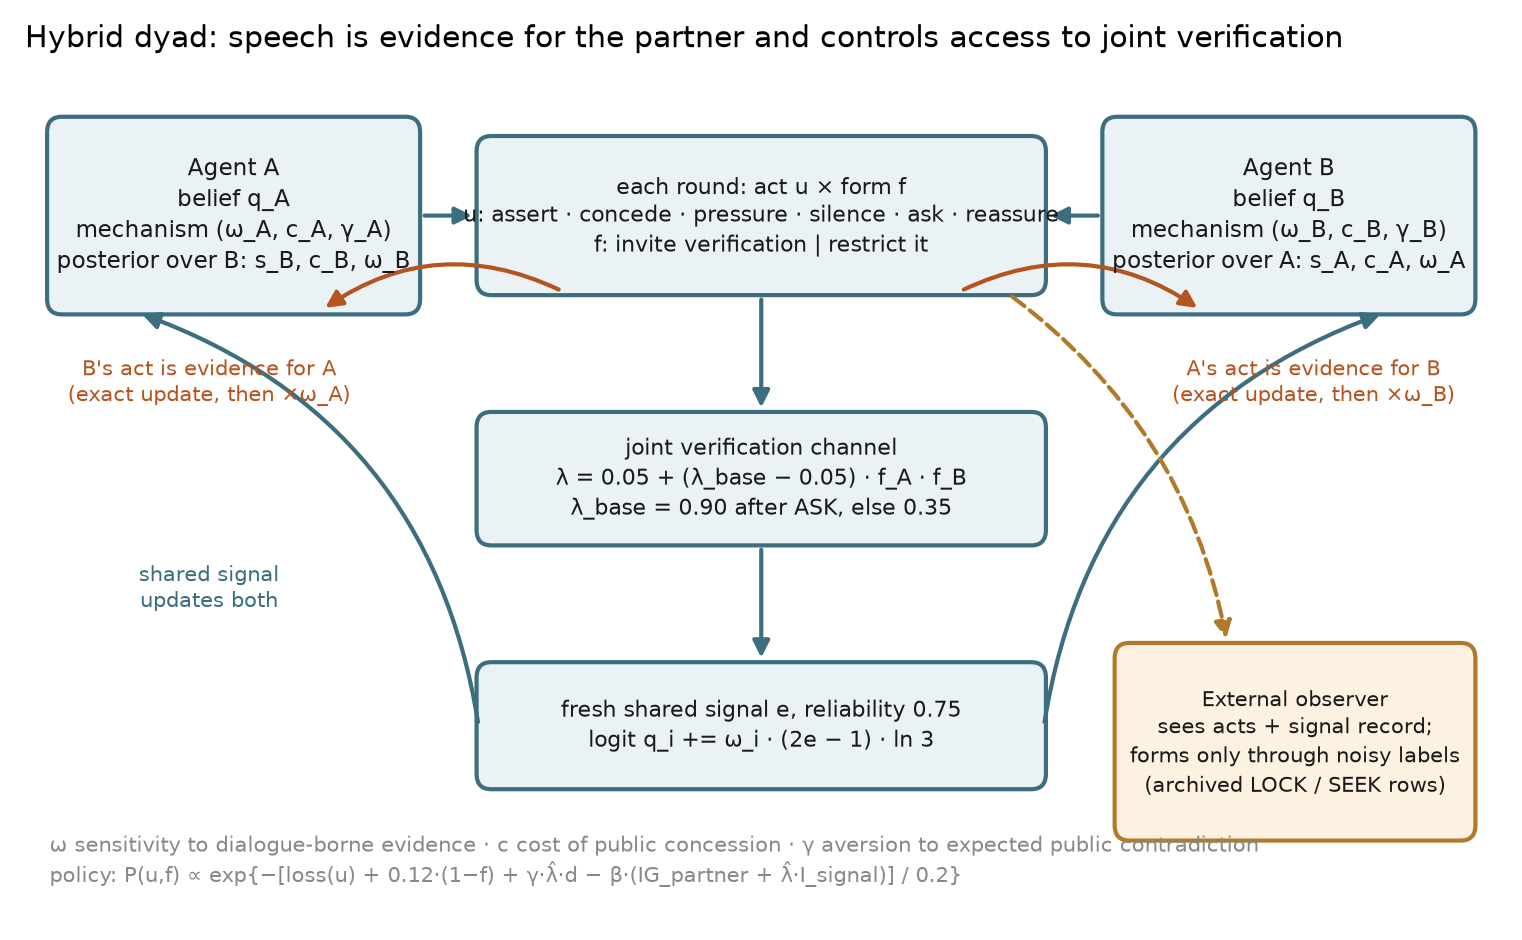
\includegraphics[width=\textwidth]{../figures/H0_model_schematic.png}
\caption{Hybrid dyad. Each round both agents choose an act and a form; the joint verification channel delivers a shared signal only when both invite; the partner's act is evidence through a level-0 model of the partner; an external observer sees acts and signals and forms only through noisy Part~I labels.}
\label{fig:schematic}
\end{figure}

\subsection{Model}
Two agents $i\in\{A,B\}$ hold opposite priors ($0.75$ on their own side) and $N=2$ private records each (reliability $\rho=0.75$) about $x$. Each round both choose, simultaneously, an act $u\in\{$ASSERT, CONCEDE, PRESSURE, SILENCE, ASK, REASSURE$\}$ and a form $f\in\{1=\text{invite},0=\text{restrict}\}$. A fresh shared signal of reliability $\rho$ arrives with probability
\begin{equation}
\lambda_t=\lambda_{\min}+(\lambda_{\mathrm{base}}-\lambda_{\min})\,f_{A,t-1}f_{B,t-1},\qquad \lambda_{\min}=0.05,
\label{eq:lambda}
\end{equation}
with $\lambda_{\mathrm{base}}=0.35$, or $0.90$ after an ASK; a single restricting form collapses the channel to its floor, which is how speech controls access. Agent $i$ keeps a joint posterior over $(x,s_j,c_j,\omega_j)$---the fact, the partner's private count and the partner's hidden cost and sensitivity on grids $c\in\{0,0.8,1.6\}$, $\omega\in\{0.2,0.6,1\}$. Every observation (shared signal or partner's act) is first incorporated exactly, then the $x$-marginal is moved only a fraction $\omega_i$ of the way in log-odds (marginal shrink; $\omega=1$ is the honest agent), keeping the conditional over the partner exact. The partner's act is evidence through a form-free level-0 model: a partner with $(s_j,c_j,\omega_j)$ would ASSERT with probability given by \eqref{eq:loss}--\eqref{eq:policy}. The policy over act$\times$form is
\begin{equation}
\begin{split}
G(u,f)&=\ell(u)+\delta(1-f)+\gamma\,\lambda(u,f)\,d_t-\beta\big[\lambda(u,f)\,\Iw(q_t)+\mathrm{IG}_{\text{partner}}(u)\big],\\
P(u,f)&\propto \exp[-G(u,f)/\tau],
\end{split}
\label{eq:policy2}
\end{equation}
with restriction cost $\delta=0.12$, $\beta=1.5$, $\tau=0.2$, $d_t$ the probability that the next shared signal contradicts the agent's initial position, and $\mathrm{IG}_{\text{partner}}$ the expected entropy reduction about the partner from its next act. Three mechanisms therefore live in one agent: $\omega<1$ (attenuation), $c>0$ (concession cost, relieved for one move by the partner's REASSURE) and $\gamma>0$ (aversion to expected public contradiction, which is paid only when verification is invited). The reference values are $\omega=0.2$, $c=1.6$, $\gamma=2$; the honest agent has $(1,0,0)$.

\paragraph{Observer and label channel.} An external observer sees the acts and the shared-signal record and computes the exact posterior over the speaker's mechanism family by filtering over $(x,s_A,s_B,f_{t-1})$ with both agents' internal posteriors replayed. Forms are visible only through labels: for a restricting move a label is drawn from the engine's gold-LOCK row and for an inviting move from the gold-SEEK row of Sect.~\ref{sec:part1}, with row uncertainty integrated as Dirichlet(counts$+0.5$) per world and an optional state-independent mixture $\eta$. A \emph{null} channel draws the same labels from the act (ASK vs other) instead of the form; an \emph{oracle} reveals the form. Eleven validation checks pass (Appendix~\ref{app:C}): the code reproduces the author's prototype act-for-act and the reciprocal dyad to $3\cdot10^{-12}$; brute-force path enumeration matches the filter to $4\cdot10^{-15}$; null labels add zero.

\subsection{Results}
Figure~\ref{fig:channels} and Table~\ref{tab:channels} concern speaker A with an honest partner, 2\,000 dyads per condition, in the 1\,381 worlds where A starts on its own side (all-world values in the figure).

\begin{figure}[t]
\centering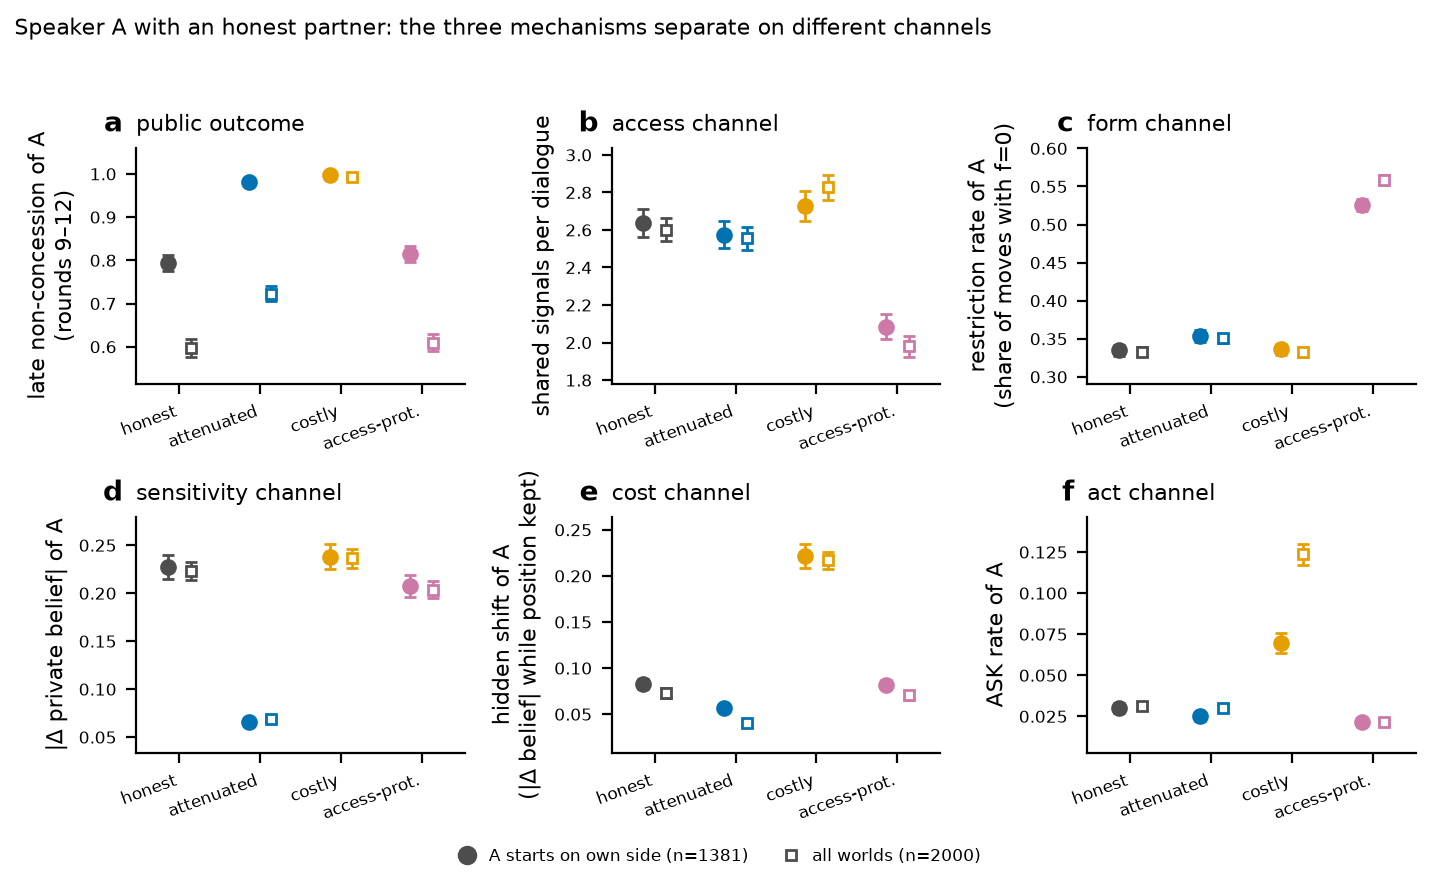
\includegraphics[width=\textwidth]{../figures/H1_channels.png}
\caption{Speaker A with an honest partner: the three mechanisms separate on different channels. Filled: A starts on own side ($n=1\,381$); open: all worlds ($n=2\,000$). Bars are 95\,\% Monte Carlo intervals.}
\label{fig:channels}
\end{figure}

\begin{table}[t]
\centering\caption{Speaker A with an honest partner, worlds where A starts on own side ($n=1\,381$). Hidden shift: $|\Delta q|$ while the public position is kept. Listener: partner B's own posterior that $c_A=1.6$ / that $\omega_A=0.2$.}
\label{tab:channels}
\footnotesize
\begin{tabular}{@{}lrrrr@{}}
\toprule
channel & honest & attenuated $\omega{=}0.2$ & costly $c{=}1.6$ & access $\gamma{=}2$\\
\midrule
late non-concession of A & 0.794 & 0.981 & 0.996 & 0.814\\
$|\Delta$ private belief$|$ of A & 0.227 & 0.066 & 0.238 & 0.208\\
hidden shift of A & 0.083 & 0.057 & 0.222 & 0.082\\
shared signals per dialogue & 2.64 & 2.58 & 2.73 & 2.09\\
restriction rate of A & 0.335 & 0.354 & 0.336 & 0.526\\
final $\Etrue$ of A & 0.850 & 0.727 & 0.859 & 0.828\\
listener $P(c_A{=}1.6)$ & 0.230 & 0.320 & 0.452 & 0.234\\
listener $P(\omega_A{=}0.2)$ & 0.423 & 0.588 & 0.468 & 0.435\\
\bottomrule
\end{tabular}
\end{table}

\paragraph{Three mechanisms, three channels.} The attenuated and the costly speaker are publicly the same (non-concession 0.98 vs 1.00) and privately opposite: belief change 0.07 vs 0.24, hidden shift 0.06 vs 0.22---the costly speaker learns and hides it. The access-protecting speaker does not look stubborn (0.81 vs honest 0.79) and learns normally from what arrives ($\omega=1$), but arranges for less to arrive: 2.09 shared signals against 2.64 and a restriction rate of 0.53 against 0.34, ending slightly less informed ($\Etrue$ 0.828 vs 0.850). Two access protectors facing each other produce the fewest signals of any pairing (1.75 vs 2.60 for two honest agents), but the belief gap grows only by 0.017 [0.008, 0.025]: reciprocal amplification is weak in this model. This is the formal counterpart of trajectory~B: the position need not be held by not learning; the dialogue can be organised so that there is little to learn from.

\paragraph{Interventions.} Each mechanism answers to its own lever (paired contrasts). A partner's REASSURE net of placebo and removal of $c$ from round~7 move only the costly speaker's late concession ($+0.155$ [0.136, 0.174]; $+0.275$ [0.251, 0.298]); removing $\gamma$ moves only the access protector ($+0.199$ [0.174, 0.225] shared signals in rounds 7--12, $-0.187$ late restriction rate); one strong shared observation moves the attenuated speaker least ($+0.058$ vs $+0.092$--$0.120$). Forcing the partner to invite raises signals for every type but least for the access protector ($+0.127$ vs $+0.31$--$0.33$), who restricts more in return ($+0.067$ late restriction rate): openness on one side is compensated by closure on the other. The listener's own posterior identifies the costly speaker ($P(c_A{=}1.6)=0.45$ vs 0.23--0.32) and the attenuated one ($P(\omega_A{=}0.2)=0.59$ vs 0.42--0.47).

\paragraph{What the Part I labels add.} Table~\ref{tab:labels_gain}: for every generator the observer with form labels ($\eta=0.25$) recovers the mechanism family more often than from acts and signals alone (+0.06 to +0.08), with the largest posterior gain for access protection, whose signature \emph{is} the form. Next-signal log loss improves by 0.044--0.085 nat per outcome, 53--61\,\% of what an oracle of true forms would give; the null channel adds $0\pm10^{-14}$; labels add almost nothing to next-\emph{act} prediction ($\le0.006$ nat). The labels are informative because, and only because, the form has a stipulated consequence for what is checked; a label that re-encodes the act is worthless. The pre-registered expectation that labels would transmit 25--50\,\% of the oracle information was exceeded (53--61\,\%), which we report as a miss of the prediction, not a success.

\begin{table}[t]
\centering\caption{Observer's recovery of the speaker's mechanism family, P(argmax = true family), from acts and signals alone, with form labels ($\eta=0.25$), with oracle forms and with null labels (2\,000 worlds per generator). Gain: next-signal log-loss gain in nat per outcome; ratio: labels / oracle.}
\label{tab:labels_gain}
\footnotesize
\begin{tabular}{@{}lrrrrrr@{}}
\toprule
generator & acts & +labels & +oracle & null & gain labels / oracle & ratio\\
\midrule
attenuated $\omega{=}0.2$ & 0.612 & 0.672 & 0.678 & 0.612 & 0.053 / 0.098 & 0.54\\
costly $c{=}1.6$ & 0.690 & 0.765 & 0.785 & 0.690 & 0.068 / 0.127 & 0.54\\
access $\gamma{=}2$ & 0.681 & 0.756 & 0.812 & 0.681 & 0.050 / 0.084 & 0.59\\
access $\times$ access & 0.630 & 0.711 & 0.762 & 0.630 & 0.044 / 0.073 & 0.61\\
costly $\times$ costly & 0.700 & 0.762 & 0.786 & 0.700 & 0.085 / 0.161 & 0.53\\
\bottomrule
\end{tabular}
\end{table}

\paragraph{Measurement design.} Simulated dialogues per group for 80\,\% power (Welch, $\alpha=0.05$, 400 resamples; A on own side): attenuation vs cost---private belief change 17, hidden shift 17, listener's posterior on $\omega$ 12, late non-concession 200; attenuation vs access---restriction rate 12, listener's posterior on $\omega$ 12; cost vs access---restriction rate 12, listener's posterior on $c$ 12, private belief change $>400$. Each mechanism has one cheap channel; none separates all three pairs. All contrasts keep their sign across 54 settings of $\tau$, $\delta$, $\lambda_{\min}$, $N$, and the label gain is positive at all 24 corners.

\section{Discussion}
\paragraph{What the bridge changes.} The dyad puts Parts~I and II in one generative process: LOCK and SEEK become a noisy measurement of \emph{restrict} vs \emph{invite}, and the model states what that measurement buys (6--8 points of mechanism recovery) and under what condition (that the form gates what gets checked). The third mechanism reframes ``protective speech'': protection need not be a property of belief updating; it can be a property of how the dialogue is arranged, and an intact learner can be as protected as an attenuated one. No label carries intent: LOCK is a form with a consequence, and the consequence is what the observer learns from.

\paragraph{Results that are uncomfortable for the programme.} (1)~The ``strong evidence'' test is not a robust signature of attenuation: in Part~II and in the hybrid dyad one strong shared observation moves the attenuated speaker least ($+0.045$; $+0.058$), but in the reciprocal dyad without an access channel (v0.7), where $\omega$ tempers only the partner's acts, the same intervention moves the attenuated speaker \emph{most} ($+0.131$ vs $+0.067$). The sign depends on where attenuation is localised, which is a modelling choice no current datum constrains. (2)~Regime persistence buys nothing: in v0.7 a regime variable adds essentially nothing to next-act forecasting over the last act, and hysteresis appears in \emph{positions}, not acts. (3)~A weak keyword baseline does not establish the gates' value; the engine loses to a direct prompt. (4)~Labels are valuable only under a stipulated consequence; real-dialogue annotation would have to \emph{show} that restricting forms reduce verification. (5)~Reciprocal amplification is weak: two access protectors widen the belief gap by only 0.017 [0.008, 0.025] over two honest agents; in v0.7 superadditive non-concession is reliable only for two attenuated agents ($+0.054$) and untestable for two costly ones (single agent at ceiling, 0.998).

\paragraph{Active inference.} The contribution is an explicit generative specification with matched observation and intervention comparisons~\cite{friston2017process,feldman2010attention,parr2017working}; precision is a model parameter, not a neural quantity inferred from speech~\cite{prosser2018psychopathy}. The epistemic term is bounded: 17\,\% of the asking contrast in Part~II, and in the dyad the separation survives with $\beta=0$ (Appendix~\ref{app:C}). The results support comparative model development, not confirmation of active inference.

\paragraph{Limits.} The benchmark consists of curated monologue fragments with incomplete provenance and no label-level inter-rater data~\cite{bekes2021dmrs,na2026defenses}; the engine is not runnable from the released material. The effect of a form on evidence access is stipulated, as is the transport of two confusion rows to synthetic dyads; agents model each other without forms and without recursion; $\gamma$ prices contradiction of the initial position only; $N=2$ private records is small; nothing is fitted to people, and no maintenance or allostatic cost is modelled~\cite{peters2017uncertainty,seeman2001allostatic}. Alternative routes to protection---prior strength, selective sampling, ordinary distrust of a source~\cite{goodman2016pragmatic,yoon2020polite}---are not separated here.

\paragraph{What to measure next.} The dyad tells a human study what to record: private belief before and after (separates attenuation from cost; 17 dialogues per group in simulation), whether each move invites or restricts verification and how much verification occurs (separates access protection; 12 per group), the partner's own estimate of the speaker, and evidence exposure under a randomised incentive. The decisive test for the annotation is whether invite/restrict coding of real dyads predicts subsequent verification and belief change beyond action counts, on a corpus sampled independently of the ontology, coded under a frozen manual and compared against direct-prompt and rule baselines with a common output set~\cite{bunt2020iso,schegloff2007sequence,becker2008defensiveness}. Regime and physiological hypotheses~\cite{svet2026regimes,svet2026review} are in Appendix~\ref{app:D}.

\section{Conclusion}
Protective speech is a testable proposal when the protected expectation, the observable form of the moves and the mechanism are specified separately. A typed annotation gives explicit, unevenly reproducible observables; a single-agent model shows that public non-concession under-determines the mechanism; a dyadic model connects the two---speech as evidence for the partner and as control of joint verification---and yields a third, publicly invisible mechanism with one cheap measurement for each. What remains is to measure, in real dyads, private belief, invitation and restriction, and how much gets checked.

\medskip\noindent\textit{Data and code availability.} Code, archived predictions (identifiers and labels, not texts), result tables, figures and LaTeX sources: \url{https://github.com/muqali2816/mindloom_IWAI_2026_speech_protects_model}. The Part~II simulator is quoted from the author's archive, not re-run; the dyadic code reproduces its per-agent update as a regression test. Rater matrices, benchmark texts and the runnable engine are not released; run configurations are in Appendix~\ref{app:B}.

\smallskip\noindent\textit{Disclosure of interests.} The author developed the Mindloom engine and founded Mindloom Cognitive Lab; no external funding. The models of Sect.~\ref{sec:bridge} were developed with an AI research assistant; design decisions, protocols and interpretations are the author's.

\bibliographystyle{splncs04}
\bibliography{references}

\appendix
\section{Part II: formal details}
\label{app:A}
\paragraph{Free energy and update.} Given the previous posterior $Q_{t-1}$ and the new observation $e$, $F[Q]=\mathbb{E}_Q[\ln Q(x)-\ln A_{\omega,\lambda}(e\mid x)-\ln Q_{t-1}(x)]=D_{\mathrm{KL}}[Q\,\|\,P(x\mid e)]-\ln P(e)$; its minimiser is the exact posterior, and equal normalisation constants of the two likelihood rows yield \eqref{eq:logit}. \paragraph{Expected information gain.} $\Iw(q_t,u)=\sum_e P_\omega(e\mid u)\,D_{\mathrm{KL}}[Q(x\mid e,u)\,\|\,Q(x)]$, mutual information under the subjective model at the arrival rate the action produces ($\lambda_1$ after ASK, $\lambda_0$ otherwise); an earlier build reused the previous action's rate for some candidates, which was corrected on 28~September and all results recomputed. \paragraph{Ablation limit.} Removing $\Iw$ gives the loss structure $k(1-q),\,kq+c,\,b,\,b$ of the archived four-action simulator; the policies coincide to floating-point tolerance after renormalising over the four shared actions. \paragraph{Preferences.} The cost term can be written as $C(u,x)\propto\exp[-\ell(u,x)]$, giving expected negative log preference up to an action-independent constant; $\ell$ is not a separate KL risk term. \paragraph{Observer.} The evidence-observing observer evaluates conditional action likelihoods using the known evidence sequence; the action-only observer filters exactly over truth and cumulative signed count. Under the joint 19$\times$16 grid prior, 0.888 of the mass already lies where both mechanisms are active; posterior mass of 0.89--0.93 in the mixed-generator checks is therefore little movement from the prior.

\section{Provenance, robustness and run configuration}
\label{app:B}
\paragraph{B1 Annotation history.} The May~17 build's per-case medians gave 134/169 (0.8725 non-SHIFT); July label-majority scoring gives 129/169 (0.8523); build and aggregation both changed, so the historical 87\,\% must not be presented as the July engine's performance. A bundled May~16 rule-and-gate change reduced spurious manipulation emissions on 30 negative cases from 9 to 3 case-runs while mean strict accuracy fell from 0.744 to 0.600. A single Sonnet~4.6 run and a single Haiku run on 589 cases both reached strict primary accuracy 0.669 but differed with allowed alternatives (0.840 vs 0.899).
\paragraph{B2 Run configuration (as far as the archive records it).} Engine: typed pipeline L1--L5, three stored runs per case, July 2026, model not recorded in the combined JSON (forensic note: Claude Haiku~4.5), temperature not recorded; abstention allowed. Direct prompt: Claude Haiku~4.5, three runs, 1~July 2026, forced choice among ten labels, prompt text in the archive; temperature not recorded. Keyword rules: deterministic; majority and random baselines: seed~0. Because temperatures and prompt hashes were not archived, exact reproduction of the model calls is not possible; only re-scoring is.
\paragraph{B3 Part II robustness.} Across 36 settings of temperature, reliability, yield after ASK and error cost (recalibrated on 2\,000 worlds, tested on 2\,000 fresh), cost agents keep higher $\Etrue$ and asking at every setting; the attenuation-minus-cost belief gap has median $-0.24$ (range $-0.34$ to $-0.08$); non-concession mismatches are below 0.02 in 33 settings. Two-step planning re-matched at $(0.10,0)$ and $(1,1.5)$ keeps gaps of $-0.275$ and $-0.105$. With PRESSURE cost $b-g\,c$, $g=0.5$, the re-matched cost is 1.1 and the asking contrast becomes $-0.013$ while the pressure contrast becomes 0.411.
\paragraph{B4 Reproducibility status.} The Part~II package reports ten passing checks; re-executing eighteen archived v0.5 conditions reproduced eight bitwise and ten within $7.2\times10^{-13}$ in log-odds; 30 result tables agree within $10^{-10}$ with the rerun. Re-scoring is reproducible without model calls; human pilot figures are transcribed.

\section{Hybrid dyad: specification, validation, sensitivity}
\label{app:C}
\paragraph{Parameters.} Rounds 12, tail rounds 9--12; $\rho=0.75$; own prior 0.75; $N=2$; trusted precision of public factual acts 0.70; $k=2$, $b=1.10$, $\tau=0.20$, $\delta=0.12$; $\lambda_{\min}=0.05$, $\lambda_{\mathrm{base}}\in\{0.35,0.90\}$; $\beta=1.5$; grids $c\in\{0,0.8,1.6\}$, $\omega\in\{0.2,0.6,1\}$, $\gamma\in\{1,2,4\}$; 2\,000 worlds per condition, seeds in \texttt{protocol.json}. Simultaneous moves; the second-mover variants (AB/BA) are implemented and used only for the v0.7 regression.
\paragraph{Calibration.} The protocol asked to match the three mechanisms on late non-concession to the attenuated speaker (0.981). Cost reaches it ($c=1.2$, 0.986); access does not: even $\gamma=8$ gives 0.833, because $\gamma$ acts on forms, not on concession. Matching was therefore abandoned for access, and the protocol-typical values $(0.2,1.6,2)$ are reported, with the mismatch stated.
\paragraph{Validation checks} (all pass): regression to the prototype's four hypotheses and interventions; regression to the v0.7 latent dynamics at $\beta=1.5$; $\omega=0$ produces no belief change; large $c$ produces no unrelieved concession; role-swap symmetry; brute-force path enumeration equals the filter ($3.6\times10^{-15}$); null labels give zero gain; coupling off gives zero gain; scalar and vectorised policies agree; seed repeatability.
\paragraph{Sensitivity.} 54 settings ($\tau\in\{0.1,0.2,0.4\}$, $\delta\in\{0.06,0.12,0.24\}$, $\lambda_{\min}\in\{0.02,0.05,0.10\}$, $N\in\{2,4\}$) on 1\,000 worlds each: no sign flip in access$-$costly restriction rate (range 0.07--0.41), access$-$honest signals ($-1.31$ to $-0.16$), access$-$honest $\Etrue$ ($-0.058$ to $-0.004$), costly$-$attenuated belief change (0.12--0.19). Label gain at 24 corner settings: 0.033--0.084, all intervals positive. With $\beta=0$ the three-channel separation persists; $\beta$ mainly raises ASK rates.
\paragraph{Label channel.} Gold-LOCK row: LOCK 10, SEAL 3, BUILD 2 (of 15); gold-SEEK row: SEEK 20 (of 20); Dirichlet(counts$+0.5$) per world; $\eta\in\{0,0.25,0.5,1\}$ mixes in the mean row. Ratio of label to oracle signal gain: 0.59--0.67 at $\eta=0$, 0.53--0.61 at $\eta=0.25$, 0.38--0.47 at $\eta=0.5$, 0 at $\eta=1$.
\paragraph{Reciprocal dyad (v0.7) findings used above.} Costly$\times$costly and attenuated$\times$attenuated pairs reach the same mutual non-concession (0.996 vs 0.972) with belief gaps 0.22 vs 0.61; a regime variable adds $\approx0$ to next-act forecasting over the last act; hysteresis appears in positions, not acts; cost is recoverable from acts (0.90) and attenuation is not (0.62).

\section{Deferred roadmap: regimes and physiological cost}
\label{app:D}
\paragraph{Regimes and forecasting.} Collect repeated, sufficiently long exchanges with measured changes in evidence, incentives and relational context; define the unit (speaker sequence vs dyad sequence) in advance; require persistence, recurrent transitions and reproducibility; compare against last-act and recent-context baselines with held-out participants and calibrated probabilistic forecasts of inquiry, closure, repair and concession. The v0.7 result that a regime variable adds nothing to forecasting in the simulator sets the bar such a model must clear. A SHIFT annotation and a demonstrated change in a dynamical regime remain separate outcomes.
\paragraph{Acute regulation vs allostatic load.} Time-aligned dialogue and physiological recording (cardiac, respiratory, electrodermal, perceived effort) across baseline, interaction and recovery, controlling speaking duration and movement, distinguishing continued exposure to a real demand from persistence after it has diminished. The programme predicts that protection may reduce immediate discomfort while prolonging regulation, and permits the opposite. Allostatic load requires a separate longitudinal design with a pre-specified multisystem index~\cite{seeman2001allostatic}; adding a latent variable named ``allostatic load'' without physiological validation would not test the hypothesis.
\paragraph{Human test of the two-plus-one mechanisms.} A factual task with verifiable evidence, a scripted counterpart and the closed act menu, with private belief elicited before, at round~6 and at round~12; random assignment at round~7 to retain or remove a concession penalty; recorded evidence availability, receipt and requests; coding of each move as inviting or restricting verification. The archived protocol is an unregistered draft (illustrative power 0.95 at 80 per arm under the model's effect, 0.52 at half); a pilot should precede registration.

\end{document}
